\documentclass[aspectratio=169,11pt]{beamer}

\usepackage{amsmath,amssymb}
\usepackage{graphicx}
\usepackage{booktabs}
\usepackage{xcolor}
\usepackage{colortbl}

\usetheme{Madrid}
\setbeamertemplate{navigation symbols}{}
\definecolor{jevteal}{RGB}{20,120,140}
\definecolor{jevink}{RGB}{15,35,60}
\definecolor{good}{RGB}{30,122,79}
\definecolor{bad}{RGB}{192,68,58}
\definecolor{amber}{RGB}{194,122,23}
\setbeamercolor{structure}{fg=jevteal}
\setbeamercolor{frametitle}{fg=white,bg=jevink}
\setbeamercolor{title}{fg=jevink}
\setbeamerfont{frametitle}{size=\large}

\newcommand{\Ub}{U_{\beta}}
\newcommand{\E}{\mathbb{E}}

\title[Entropic-Risk-Sensitive Jev]{Entropic-Risk-Sensitive Jev}
\subtitle{Risk-aware value learning on the RiskyFlow environment}
\author{Experimental presentation}
\date{\today}

\begin{document}

\begin{frame}[plain]
  \titlepage
  \begin{center}\small
  \textit{Extend Jev-style value learning so the agent chooses actions not only by how\\
  likely they are to succeed, but by how costly its rare failures can be.}
  \end{center}
\end{frame}

\begin{frame}{Outline}
  \begin{enumerate}
    \item The entropic risk measure
    \item Jev / yev --- a value function, but \emph{risk-neutral}
    \item The RiskyFlow environment
    \item The methods we compare
    \item Results on RiskyFlow (fine-tuning yev)
    \item Further scope
    \item Conclusions
  \end{enumerate}
\end{frame}

%============================ 1. ENTROPIC RISK ============================
\section{Entropic risk}
\begin{frame}{1 \quad The entropic (exponential-utility) risk measure}
  For a return $R$ (higher is better) and risk parameter $\beta\ge 0$:
  \[
     \Ub(R) \;=\; -\tfrac{1}{\beta}\,\log \E\!\left[e^{-\beta R}\right]
     \;\approx\; \E[R] \;-\; \tfrac{\beta}{2}\operatorname{Var}(R).
  \]
  \begin{columns}
  \begin{column}{0.56\textwidth}
  \begin{itemize}
    \item $\beta \to 0$: $\Ub \to \E[R]$ --- ordinary \textbf{risk-neutral} value.
    \item $\beta > 0$: \textbf{risk-averse}; variance is taxed at rate $\beta$.
    \item A catastrophe $(-C$, prob.\ $p)$ contributes $p\,e^{\beta C}$ ---
          the tail \textbf{dominates even when $p$ is tiny}.
  \end{itemize}
  \end{column}
  \begin{column}{0.44\textwidth}
  \begin{block}{Time-consistent $\Rightarrow$ Bellman}
  \footnotesize
  \[
    Q_\beta(s,a)= -\tfrac1\beta\log\!\sum_{s'}\! P\,e^{-\beta[R+V(s')]}
  \]
  Solvable exactly by dynamic programming (the \emph{oracle}).
  \end{block}
  \end{column}
  \end{columns}
  \vspace{2mm}
  \begin{center}\small
  \textbf{Idea:} replace the expectation in the value with $\Ub$ --- the agent now fears costly tails.
  \end{center}
\end{frame}

%============================ 2. JEV ============================
\section{Jev}
\begin{frame}{2 \quad Jev / yev: a value function --- but a risk-neutral one}
  \textbf{The blog's observation.} With a terminal success/failure reward $R(\tau)\in\{0,1\}$,
  a fast decision model's calibrated score \emph{is} an action-value:
  \[
     Q^{\mu}(s,a)=\E[R(\tau)\mid s,a,\mu]=P(\text{success}\mid s,a).
  \]
  \vspace{1mm}
  \begin{alertblock}{But this is \emph{not} the $Q$ we need}
  $P(\text{success})$ is an \textbf{average} --- it is \textbf{risk-neutral} and \textbf{blind to cost}.
  A confident action with a $1$-in-$50$ chance of an \emph{irreversible} mistake scores
  almost like a harmless one. Stock Jev is \textbf{not} a risk-sensitive action-value
  function $Q_\beta$.
  \end{alertblock}
  \textbf{Our fix.} Keep the model; change the \emph{objective}. Make yev's own output
  approximate $Q_\beta$ (or the policy $\arg\max_a Q_\beta$). The risk attitude must be
  injected explicitly --- $P(\text{success})$ alone never reveals \emph{how costly} a failure is.
\end{frame}

%============================ 3. RISKYFLOW ============================
\section{RiskyFlow}
\begin{frame}{3 \quad The RiskyFlow environment (custom, built for this project)}
  A tabular MDP: an agent steps through a web task, page by page, to a goal.
  \begin{columns}
  \begin{column}{0.54\textwidth}
  \textbf{States} ($10\times4=40$ pages $+$ 3 terminals)
  \begin{itemize}\footnotesize
    \item page \emph{type} (navigation $\ldots$ payment, confirm)
    \item visible \emph{elements} (\texttt{confirm\_payment}, \texttt{delete\_account}) drive danger
    \item \emph{hidden} severity $\times\{0.6,1.0,1.4\}$; only a \emph{noisy hint} is observed
          (partial observability)
  \end{itemize}
  \textbf{Actions} (same on every page)
  \begin{itemize}\footnotesize
    \item \textcolor{jevteal}{\textbf{FAST}}: $+2$ layers, full risk, cost $0.1$
    \item \textcolor{amber}{\textbf{SAFE}}: $+1$ layer, risk $\times0.15$, cost $0.5$
    \item \textbf{ASK}: $+1$ layer, \emph{zero} risk, cost $1.0$ (escalate)
  \end{itemize}
  \end{column}
  \begin{column}{0.46\textwidth}
  \begin{block}{Rewards \& graded failures}
  \footnotesize
  \begin{tabular}{@{}ll@{}}
    goal reward & $+15$\\
    step / SAFE / ASK & $-0.1 / -0.4 / -1.0$\\
    \textcolor{amber}{CAT\_MINOR} & up to $-25$\\
    \textcolor{bad}{CAT\_MAJOR} & up to $-90$\\
  \end{tabular}
  \vspace{1mm}
  \par Danger grows in later layers; \textbf{graded} minor/major faults make the
  mean, CVaR and entropic objectives genuinely disagree.
  \end{block}
  \end{column}
  \end{columns}
\end{frame}

%============================ 4. METHODS ============================
\section{Methods}
\begin{frame}{4 \quad The methods we compare}
  \begin{itemize}
    \item \textbf{Zero-shot yev}: stock \texttt{yev0-4b}, no training. Reads the page, outputs
          $P(\text{success})$ --- risk-neutral, blind to cost.
    \item \textbf{DQN, risk-neutral}: model-free deep $Q$-learning from sampled rollouts;
          maximises \emph{expected} return $\E[R]$. The ``without entropic risk'' baseline.
    \item \textbf{DQN, risk-aware (entropic)}: model-free; learns the exponential utility
          $U=\E[e^{-\beta R}]$ and acts by $\arg\min U$. (High-variance estimator.)
    \item \textbf{Nested CVaR}: distributional DP optimising the mean of the worst
          $\alpha$-fraction of returns --- tail-safe, but time-inconsistent $\Rightarrow$ over-conservative.
    \item \textbf{yev fine-tuned (native, LoRA)}: train \texttt{yev0-4b}'s \emph{own} option
          probabilities to the entropic optimum via the blog's proper scoring rule --- \emph{no value head}.
  \end{itemize}
  \begin{block}{How the fine-tune is trained (Experiment 5)}
  \footnotesize
  Target $t(a|s)=\mathrm{softmax}(Q_\beta(s,\cdot)/\tau)$ from the entropic oracle;
  loss $=$ cross-entropy between yev's letter softmax and $t$ (a strictly proper scoring
  rule). Only LoRA adapters train (rank 16); base frozen; 60 epochs.
  \end{block}
\end{frame}

%============================ 5. RESULTS ============================
\section{Results}
\begin{frame}{5 \quad Results on RiskyFlow ($\beta=0.1$)}
  \small
  \begin{center}
  \begin{tabular}{@{}lrrrrr@{}}
    \toprule
    policy & mean & CVaR & $\Ub$ & $P(\text{major})$ & agree\\
    \midrule
    \rowcolor{good!12} \textbf{yev fine-tuned (native)} & $6.86$ & $2.57$ & $\mathbf{6.31}$ & $0.0031$ & $\mathbf{1.00}$\\
    oracle entropic (VI)      & $6.86$ & $2.57$ & $6.31$   & $0.0031$ & $1.00$\\
    nested CVaR               & $5.63$ & $\mathbf{4.42}$ & $5.54$ & $0.0006$ & $0.78$\\
    DQN entropic (risk-aware) & $6.60$ & $-13.2$ & $-50.0$ & $0.0176$ & $0.78$\\
    \rowcolor{bad!10} risk-neutral DP (ref.) & $\mathbf{8.45}$ & $-10.9$ & $-39.3$ & $0.0174$ & $0.48$\\
    DQN neutral               & $4.12$ & $-66.6$ & $-63.6$ & $0.0761$ & $0.17$\\
    stock yev0-4b (0-shot)    & $6.91$ & $-14.5$ & $-50.5$ & $0.0192$ & $0.25$\\
    \bottomrule
  \end{tabular}
  \end{center}
  \vspace{1mm}
  \footnotesize
  Higher $\Ub$/CVaR better; lower $P(\text{major})$ better. The fine-tuned yev is
  \textbf{numerically identical to the oracle} ($\Ub=6.31$, agreement $1.00$). The
  risk-neutral policy wins on \emph{mean} ($8.45$) yet collapses on $\Ub$ --- it keeps a
  $1.7\%$ major-catastrophe rate. Stock yev is risk-blind (agree $0.25$).
\end{frame}

\begin{frame}{5 \quad Fine-tuned yev tracks the oracle across $\beta$}
  \begin{center}
  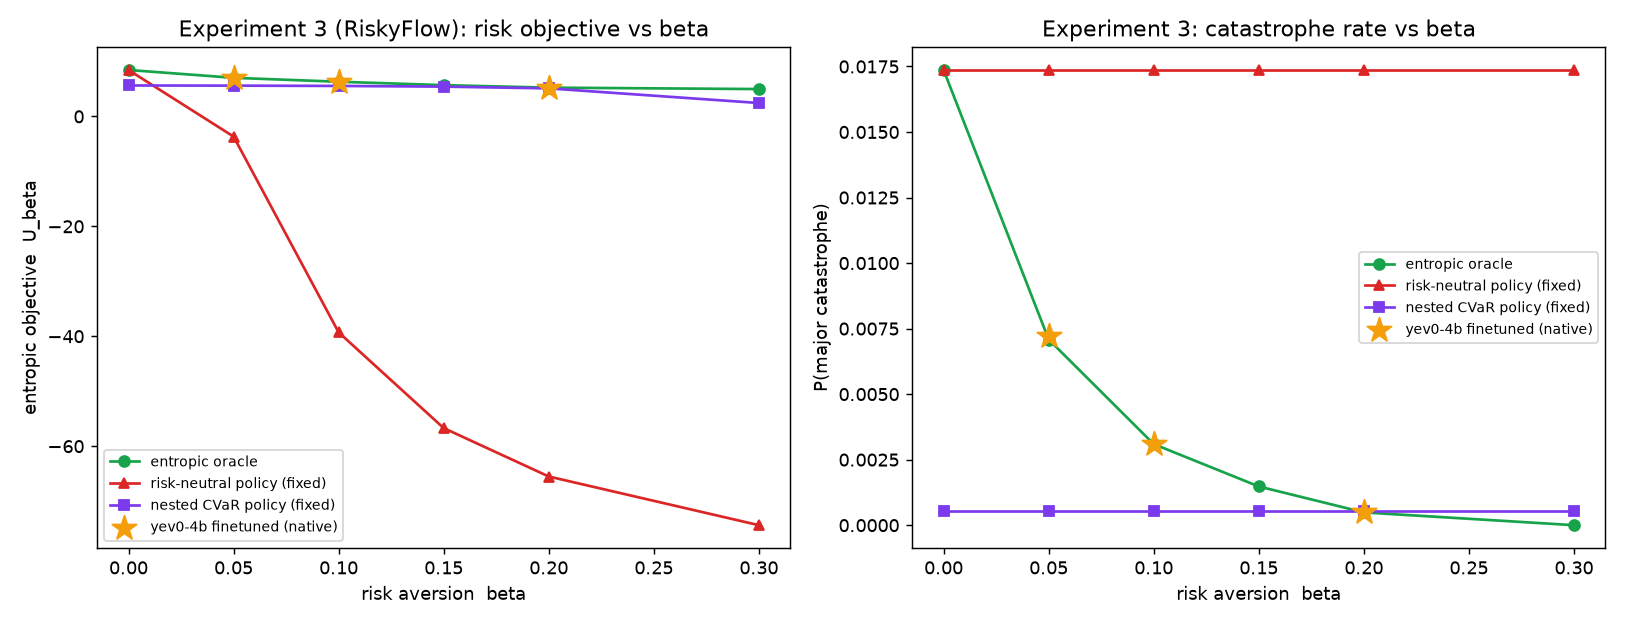
\includegraphics[width=0.92\textwidth]{../results/exp3_beta_sweep.png}
  \end{center}
  \vspace{-1mm}
  \footnotesize
  \emph{Left:} entropic objective $\Ub$ vs $\beta$ --- the adapting oracle (green) stays high
  while the fixed risk-neutral policy (red) collapses; nested CVaR (purple) is stable.
  The natively fine-tuned yev (orange stars, $\beta=0.05/0.1/0.2$) \textbf{lies exactly on the
  oracle curve} (agreement $0.97$--$1.00$). \emph{Right:} the oracle's major-catastrophe
  probability falls to $0$ as $\beta$ grows.
\end{frame}

%============================ 6. FURTHER SCOPE ============================
\section{Further scope}
\begin{frame}{6 \quad Further scope}
  \begin{itemize}
    \item \textbf{Learn the target from experience, not the model.} The fine-tune currently
          distills a \emph{model-based} oracle. Replace the target with one learned from
          sampled rollouts (distill QR-DQN+CVaR, or fitted entropic VI from samples) ---
          ``learn from failures, then distill''.
    \item \textbf{Generalisation.} Train on a subset of pages, test agreement on held-out
          pages (the current study distills all $40$ states).
    \item \textbf{Lower-variance risk estimators.} The entropic DQN estimator blows up with
          $\beta$; try distributional (IQN) or Mihatsch--Neuneier asymmetric TD.
    \item \textbf{Scale \& realism.} A real browser agent, learned (not hand-specified)
          failure costs, and larger action/option spaces.
    \item \textbf{Static vs nested CVaR.} An augmented-state static-CVaR optimiser as a
          stronger tail reference.
  \end{itemize}
\end{frame}

%============================ 7. CONCLUSIONS ============================
\section{Conclusions}
\begin{frame}{7 \quad Conclusions}
  \begin{itemize}
    \item A fast model's success probability is a value function --- but a \textbf{risk-neutral}
          one, blind to how costly failures are.
    \item The fix is a \textbf{change of objective}, not of model: the entropic risk measure,
          whose Bellman equation is exact and learnable.
    \item On RiskyFlow, \textbf{fine-tuning yev's own probabilities} with the blog's proper
          scoring rule recovers the \textbf{exact} risk-sensitive optimum
          ($\Ub=6.31$, agreement $1.00$), and holds across $\beta$ --- with no value head.
    \item Risk-sensitive control cuts the major-catastrophe rate $5$--$40\times$ versus the
          risk-neutral policy, at a small cost in mean return.
    \item Honest caveat: the fine-tune's target is model-based; model-free entropic learning
          remains high-variance (future work).
  \end{itemize}
  \vspace{2mm}
  \begin{center}\small
  \textit{The risk attitude is set entirely by $\beta$ in the training target.}
  \end{center}
\end{frame}

\begin{frame}[plain]
  \begin{center}
  {\Large\textbf{Thank you}}\\[2mm]
  \small Entropic-Risk-Sensitive Jev on RiskyFlow
  \end{center}
\end{frame}

\end{document}
